\chapter{Dijkstra's Algorithm}

Edsger W. Dijkstra was a great Dutch computer scientist. He came up
with an algorithm for finding the cheapest path through a graph with
weighted edges. Today it is known as \newterm{Dijkstra's
  Algorithm}. It is used in a wide variety of common problems.  It is
also really pretty simple and elegant.\index{Dijkstra, Edsger} \index{Dijkstra's Algorithm}

\section{Algorithm Description}

You are going to mark each node with how much it would cost to get
there from some origin node.  For example, if you are shipping a
container from Long Beach, you will mark each city with the cost of
getting the container to that city.

You start by marking the price for Long Beach to zero.  (The container
is already there.)  Then, you mark each adjacent city with the cost on
the edge. Now you declare Long Beach to be ``visited''.

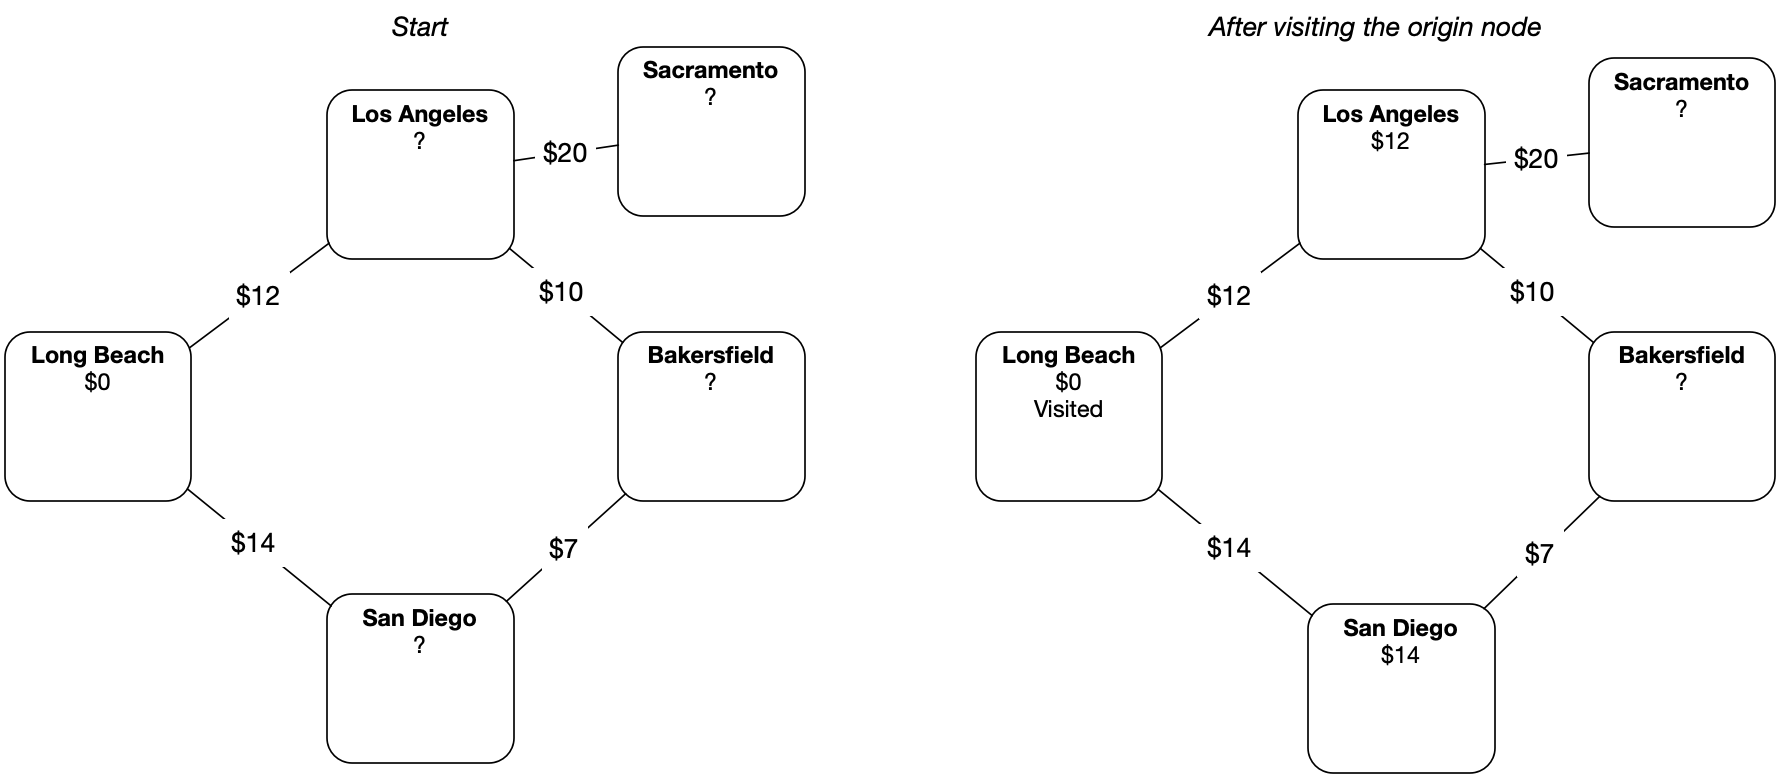
\includegraphics[width=0.9\textwidth]{step1.png}

Now, you find the cheapest of the unvisited nodes.  In this case, Los
Angeles is cheaper than San Diego, so that is the node you will visit
next.

You mark all of the unvisited nodes adjacent to Los Angeles, with the
price to ship it to Los Angeles plus the cost of shipping the
container from Los Angeles to that city. Note that Bakersfield is
marked with \$22.

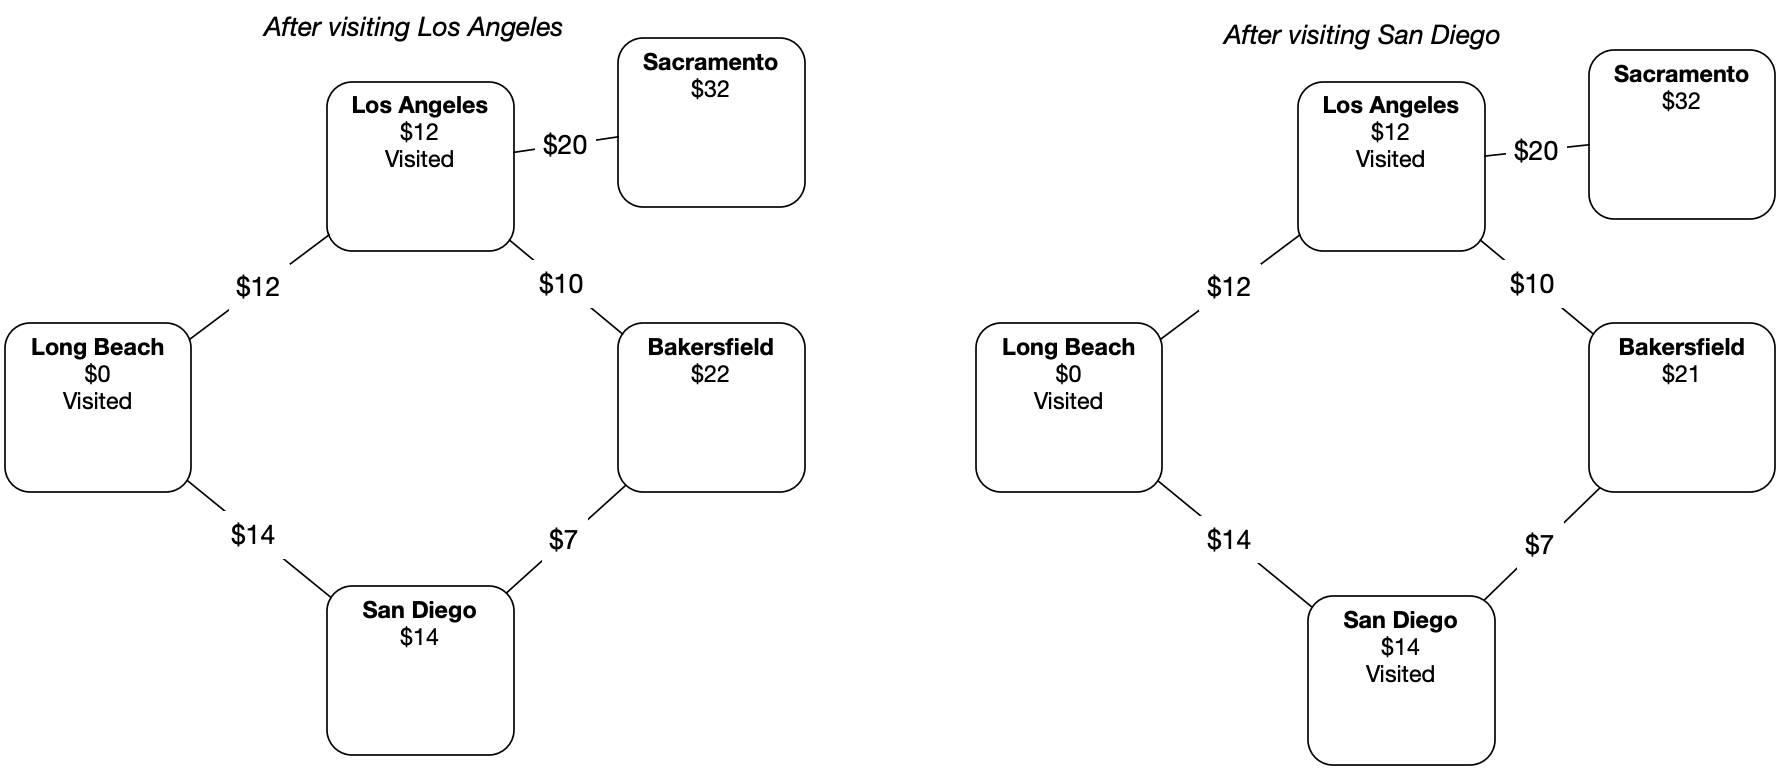
\includegraphics[width=0.9\textwidth]{step2.png}

Now the cheapest unvisited node is San Diego.  So you mark its
neighbors with the cost to ship to San Diego plus the price to ship
from San Diego to the neighbor.

Notice that Bakersfield is already labeled with \$22 from a route
through Los Angeles.  But the price would be \$21 if you shipped it to
Bakersfield via San Diego.  Because the new route is cheaper, you
change the price to the lower value.

(What does it mean that a node is ``visited''?  If a node is marked
visited, it is marked with a price that won't get any smaller.)

And you continue visiting the cheapest unvisited node until all the
nodes have been visited.  Then you know every node has been marked
with its lowest price.

In a big graph, each node may be marked several times in this process
-- each time with a lower price from a cheaper router.

Of course, once you have the price, you will ask ``What is the route
that gets me that price?''  So we will also mark each node with the
neighbor from which it would receive the shipment -- the previous
node.  This is easy to do as we execute the algorithm.

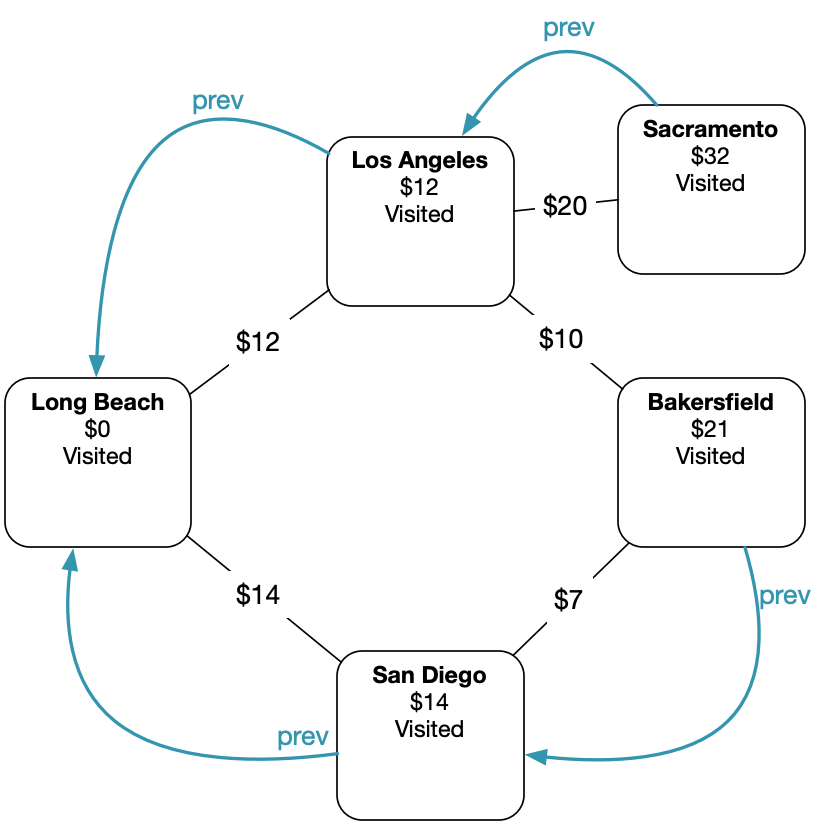
\includegraphics[width=0.4\textwidth]{prev.png}

Now, to figure out the cheapest route from San Diego to Bakersfield,
we start at the destination and follow the \pyvar{prev} pointer back
through San Diego and then to Long Beach.

\section{Implementation}

We don't actually want to sully our graph objects with the three additional pieces of information we need:
\begin{itemize}
\item The current minimal cost from the origin node. This is usually
  called the \pyvar{dist}, from ``distance''.
\item The neighbor who gives us the current minimal cost. This is
  usually called \pyvar{prev}, from ``previous''.
\item Whether the city is visited or now.
\end{itemize}
So we will keep them in collections external to the graph.

For example, to keep track of the \pyvar{dist}, we will have a
\pyvar{dist} dictionary: Each node will be a key, the current minimal
cost will be the value.  If the node hasn't received even a first
cost, we will put in infinity as the cost.

(After the algorithm is run, if the cost of a node is still infinity,
that means that it cannot be reached from the origin node.)

We will also have a \pyvar{prev} dictionary. The final node will be
the key, and its previous neighbor will be the value.

Finally, the graph has a list of all the nodes, so we can just keep a
set of the unvisited nodes.

Add a method to the \pytype{Graph} class that implements Dijkstra's algorithm:
\begin{verbatim}
    def cost_from_node(self, origin_node):
        # Cost of cheapest path from origin node discovered so far
        # Initially the origin is zero and all the other are infinity
        dist = {k: math.inf for k in self.nodes}
        dist[origin_node] = 0.0

        # The previous city on that cheapest path
        prev = {}

        # All the nodes start as unvisited
        unvisited = set(self.nodes)
    
        # While there are still unvisited nodes
        while unvisited:

            # Find unvisited node with lowest cost
            min_cost = math.inf
            for u in unvisited:
                if dist[u] < min_cost:
                    current_node = u
                    min_cost = dist[u]

            # If none are less than inf, we are done
            # This happens in graphs that are not connected
            if min_cost == math.inf:
                return (dist, prev)
            
            # Remove the lowest cost node from the unvisited list
            unvisited.remove(current_node)

            # Update all the unvisited neighbors
            for edge in current_node.edges:

                # What node is at the other end of this edge?
                v = edge.other_end(current_node)

                # Visited nodes are already minimized, skip them
                if v not in unvisited:
                    continue

                # Is this a shorter route?
                alt = dist[current_node] + edge.cost
                if alt < dist[v]:

                    # Update the distance and prev dicts
                    dist[v] = alt
                    prev[v] = current_node

        return (dist, prev)
\end{verbatim}

Append some code to your \filename{cities.py} that test this method:

\begin{verbatim}
(cost_from_long_beach, prev) = network.cost_from_node(long_beach)
print(f"\nMinimum costs from Long Beach = {cost_from_long_beach}")
print(f"\nLast city before = {prev}")

nyc_cost = cost_from_long_beach[nyc]

if nyc_cost < math.inf:
    print(f"\n*** Total cost from Long Beach to NYC: ${nyc_cost:.2f} ***")
else:
    print("You can't get to NYC from Long Beach")
\end{verbatim}

When you run it, you should get a list of how much it costs to ship a
container to each city from Long Beach:
\begin{verbatim}
Minimum costs from Long Beach = {(node:Long Beach, edges:1): 0.0,
(node:Los Angeles, edges:3): 12.0, (node:Denver, edges:3): 35.0,
(node:Pheonix, edges:3): 31.0, (node:Louisville, edges:3): 49.0,
(node:Cleveland, edges:4): 44.0, (node:Boston, edges:2): 57.0,
(node:New York City, edges:3): 52.0}
\end{verbatim}

You will also get a collection of node pairs. What are these? For each
node, you get the node that you would pass through on the cheapest
route from Long Beach:
\begin{verbatim}
Last city before = {(node:Los Angeles, edges:3):(node:Long Beach, edges:1),
(node:Denver, edges:3):(node:Los Angeles, edges:3),
(node:Pheonix, edges:3):(node:Los Angeles, edges:3),
(node:Louisville, edges:3):(node:Denver, edges:3),
(node:Cleveland, edges:4):(node:Denver, edges:3),
(node:New York City, edges:3):(node:Cleveland, edges:4),
(node:Boston, edges:2): (node:Cleveland, edges:4)}
\end{verbatim}

Your users won't want to read this; Give them the shortest path as a list.  Add a function to
\filename{graph.py} that turns the \pyvar{prev} table into a path of
nodes that lead from the origin to the destination:

\begin{verbatim}
def shortest_path(prev, destination):

    # Include the destination in the path
    path = [destination]
    current_node = destination

    # Keep stepping backward in the path
    while current_node in prev:

        # What node should come before the current node?
        previous_node = prev[current_node]

        # Insert it at the start of the list
        path.insert(0, previous_node)
        current_node = previous_node

    return path
\end{verbatim}

Test that out:

\begin{Verbatim}[commandchars=\\\{\}]
if nyc_cost < math.inf:
    print(f"*** Total cost from Long Beach to NYC: ${nyc_cost:.2f} ***")

    \textbf{path_to_nyc = graph.shortest_path(prev, nyc)}
    \textbf{print(f"*** Cheapest path from Long Beach to NYC: {path_to_nyc} ***")}
else:
    print("You can't get to NYC from Long Beach")
\end{Verbatim}

This should look like this:
\begin{verbatim}
*** Cheapest path from Long Beach to NYC: [(node:Long Beach, edges:1),
(node:Los Angeles, edges:3), (node:Denver, edges:3), (node:Cleveland, edges:4),
(node:New York City, edges:3)] ***
\end{verbatim}

\section{Making it faster}

On really big networks, doing a full Dijkstra's algorithm would take
too long. So there are a lot of methods for getting similar results
quickly.  When you ask for directions from Google Maps, it doesn't do
a full Dijkstra's Algorithm for every possible route -- it would just
take too long.

But there is a way to speed up this implementation. Look at this snippet:

\begin{verbatim}
            # Find unvisited node with lowest cost
            min_cost = math.inf
            for u in unvisited:
                if dist[u] < min_cost:
                    current_node = u
                    min_cost = dist[u]
\end{verbatim}

We are scanning through the list of all unvisited nodes, one-by-one,
looking for the one with the lowest cost.  If we kept this list sorted
by cost, then the next one to visit would always be the first one in
the list. This is done with a \newterm{priority queue} -- a list that
keeps itself sorted by some priority number -- in this case the
cost. In python, the standard priority queue is \pytype{heapq}.\index{priority queue}

(So why didn't I implement this using \pytype{heapq}? For Dijkstra's
Algorithm, the nodes' priority -- the current cost --  changes as we find
cheaper routes. \pytype{heapq} doesn't handle the changing priority
very gracefully.)

In the next chapter, you will make a priority queue class that will
work in this case.
